\chapter{Introducci\'on}\label{chap_intro}
\minitoc

\section{Biofot\'onica y nuevos m\'etodos de adquisici\'on de im\'agenes}

Uno de los avances cient\'ificos m\'as importantes del siglo \textrm{XXI} es la biofot\'onica, estudio multidisciplinario que integra cuatro tecnolog\'ias: l\'aseres, fot\'onica, nanotecnolog\'ia y biotecnolog\'ia. 

La biofot\'onica fusiona ciencias biom\'edicas con la fot\'onica y estudia interacciones entre la luz y sistemas biol\'ogicos. Cuando esta definici\'on se toma en el sentido en el que la fot\'onica se aplica en ciencias biom\'edicas, la biofot\'onica busca resolver problemas de salud en \'areas de oncolog\'ia, dermatolog\'ia, oftalmolog\'ia, cirug\'ia y cardiolog\'ia; presentando nuevas modalidades de terapias basadas en luz guiada y activadas por luz, y alternativas para la detecci\'on temprana de enfermedades.

En la figura \ref{cuadro_intro} se muestra un panorama general de las aplicaciones en biofot\'onica para el cuidado de la salud. Se han desarrollado tratamientos que simplifican la entrega de medicamentos en sitios de inter\'es y terapias capaces de destruir c\'elulas cancer\'igenas, as\'i como el desarrollo de diagn\'osticos confiables basados en diversas t\'ecnicas y dispositivos que realizan un estudio estructural de c\'elulas y tejidos.

Un \'area fundamental de la biofot\'onica est\'a enfocada en la adquisici\'on de im\'agenes $in$ $vivo$ e $in$ $vitro$ de espec\'imenes o muestras biol\'ogicas utilizando m\'etodos \'opticos. Las t\'ecnicas que se encargan de monitorear propiedades \'opticas para formar una imagen, se basan principalmente en el an\'alisis de fluorescencia, transmisi\'on y reflexi\'on de la luz, como la tomograf\'ia de coherencia \'optica, espectroscop\'ia y microscop\'ia. 

\begin{figure}[h]
\centering
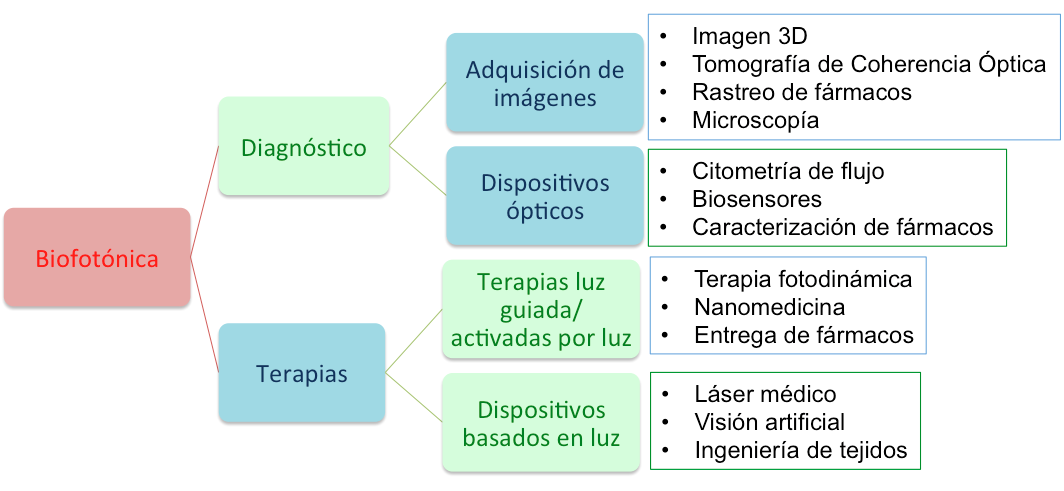
\includegraphics[width=1\textwidth]{introduccion/intro}
\caption{Alcance multidisciplinario de la Biofot\'onica en el cuidado de la salud \label{cuadro_intro}}
\end{figure}

%Por ejemplo, en la terapia fotodin\'amica se utiliza un agente qu\'imico o fotosensibilizador que al ser activado por luz destruye c\'elulas cancer\'igenas; en relaci\'on a tratamientos m\'edicos, se han desarrollado portadores de f\'armacos, que con ayuda de la nanotecnolog\'ia simplifican la entrega de medicamentos en ciertos sitios de inter\'es. Y enfocadas en el diagn\'ostico, hay t\'ecnicas en las que se utilizan marcadores fluorescentes como citometr\'ia de flujo, espectroscop\'ia de fluorescencia y dispositivos como biosensores \'opticos que pueden realizar desde un estudio estructural de c\'elulas y tejidos hasta una detecci\'on temprana de c\'ancer.

En la actualidad la microscop\'ia ha sido ampliamente utilizada debido a las im\'agenes de mayor resoluci\'on y contraste que se pueden adquirir en comparaci\'on con otras t\'ecnicas convencionales. La microscop\'ia combina e implementa t\'ecnicas como la microscop\'ia confocal, microscop\'ia de barrido y microscop\'ia de fluorescencia; adem\'as se han desarrollado microscopios basados en procesos de \'optica no lineal como la microscop\'ia de segundo o tercer arm\'onico y multifot\'on.

El desarrollo de nuevos materiales biocompatibles ha contribuido con el avance de algunas aplicaciones en biofot\'onica. Ha impulsado tratamientos, terapias y m\'etodos de diagn\'ostico, con el uso de fotosensibilizadores, portadores de f\'armacos y agentes qu\'imicos. Particularmente ha sido fundamental en t\'ecnicas de microscopia que involucran el an\'alisis de fluorescencia por el uso de compuestos qu\'imicos ex\'ogenos como marcadores en especies biol\'ogicas.

%Entre los cuales se pueden citar colorantes comerciales, nanopart\'iculas inorg\'anicas, puntos cu\'anticos y recientemente, nanoparticulas org\'anicas utilizando nuevos pol\'imeros conjugados y mol\'eculas de tama\~{n}os variables con propiedades de inter\'es.

%La carcterizaci\'on \'optica de los nuevos materiales se seleccionan cuales de ellos pueden utilizarse para solucionar problemas espec�ficos en la adquisicionnn de la imagen e s

%Se han utilizado como marcadores biocompatibles 
%no me importa esto%%%%%%%%%%%%%%\textcolor{emerald}{\sffamily This manual was made using the template that you just downloaded. All the source files are included so you can recompile, modify, and deconstruct any part of it. Text that is this color and style indicates that I am talking about this document you are reading. I believe in learning by doing \cite{oetiker2011not} so I suggest you follow along and review the source code while reading.}

\section{Antecedentes: Marcadores en microscop\'ia de fluorescencia}

Durante el siglo XVII  se llev\'o a cabo la primera observaci\'on de c\'elulas con un microscopio \'optico, desde entonces el desarrollo de nuevas t\'ecnicas y dispositivos para la obtenci\'on de im\'agenes con mayor resoluci\'on no se hizo esperar. En 1911 el f\'isico Oskar Heimst\"adt (tras el desarrollo del primer microscopio UV por August K\"ohler) construy\'o el primer microscopio de fluorescencia con el cual se visualiz\'o una bacteria \cite{revistanature}. A pesar de ello, este microscopio ten\'{\i}a una fuerte limitante: la obtenci\'on de im\'agenes depend\'{\i}a de la autofluorescencia o fluorescencia end\'ogena de los objetos.

Para ampliar los alcances de este microscopio, el austriaco Max Haitinger desarroll\'o una t\'ecnica de fluorescencia secundaria o ex\'ogena la cual implicaba el uso de qu\'{\i}micos que induc\'{\i}an fluorescencia en las muestras. En 1934 Haitinger acu\~{n}\'o el t\'ermino \emph{fluorocromo}  para referirse a estos colorantes fluorescentes \cite{libro}, aunque hoy en d\'{\i}a se conocen tambi\'en como fluor\'oforos. 

Sin embargo, el descubrimiento m\'as importante en el campo de microscop\'ia de fluorescencia se llev\'o a cabo en 1941 por Albert Coons: la inmunofluorescencia \cite{libro}. Esta t\'ecnica  permite localizar biomol\'eculas espec\'{\i}ficas en c\'elulas o tejidos, adhiriendo un colorante fluorescente a un anticuerpo (Ver Figura \ref{celfluo}). Coons localiz\'o diversos tipos de prote\'inas en c\'elulas, adhiriendo una sustancia org\'anica hidrosoluble conocida como fluoresce\'ina a un anticuerpo.


\begin{figure}[ht]
\centering
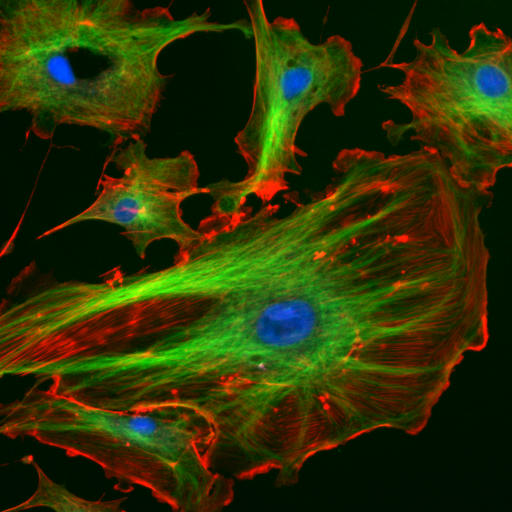
\includegraphics[width=3.2in, height=2.5in]{introduccion/FluorescentCells}
\caption{\small{C\'elulas endoteliales bajo microscopio de fluorescencia. En azul, el n\'ucleo te\~{n}ido con el colorante DAPI, en verde y rojo, los microt\'ubulos y filamentos de actina te\~{n}idos por la adhesi\'on de los colorantes FITC y TRITC en anticuerpos.} \emph{\scriptsize{Imagen obtenida de http://rsb.info.nih.gov/ij/images/, sin datos de autor.}}}\label{celfluo}
\end{figure}

Aunque algunas mol\'eculas org\'anicas como la flavina, lipofuscina, prote\'inas y coenzimas, presentan autofluorescencia y pueden ser \'utiles para monitorear procesos celulares; la microscop\'ia de fluorescencia se basa en visualizar, rastrear y/o monitorear la ubicaci\'on o patr\'on de fluorescencia en c\'elulas y tejidos que han sido marcados con fluor\'oforos ex\'ogenos \cite{procons}. 
%En estos casos la autoflorescencia es un problema de ruido que se busca resolver con los m\'etodos  anteriores de microscopia. 



La microscop\'ia de fluorescencia se ha desarrollado en las \'ultimas d\'ecadas con la implementaci\'on de diversos componentes \'opticos y marcadores biocompatibles para obtener im\'agenes de especies biol\'ogicas con resoluci\'on de hasta nan\'ometros. Actualmente hay varios m\'etodos ampliamente utilizados que se basan o pueden basarse en la microscop\'ia de fluorescencia, tales como microscop\'ia de reflexi\'on total interna, confocal,invertida y microscop\'ia de barrido l\'aser de uno y dos fotones entre otras \cite{bioph}.

%Hay un creciente inter\'es en desarrollar materiales que puedan ser utilizados como marcadores fluorescentes sin que afecten la estructura \'o el funcionamiento normal de las c\'elulas y que no causen muerte celular en presencia o ausencia de la fuente de excitaci\'on, es decir que sean marcadores $biocompatibles$.   

\section{Diferentes tipos de marcadores fluorescentes  ?`Por qu\'e utilizar nanopart\'iculas org\'anicas?}
%\subsection{A Note On Operating Systems}
 %\textbf{NEVER} 
 
Hay diversos colorantes comerciales que se pueden utilizar como marcadores biocompatibles, sin embargo, estos tienen limitantes como baja eficiencia cu\'antica de fluorescencia, una tendencia a sufrir r\'apidamente una destrucci\'on fotoqu\'imica conocida como fotoblanqueado (photobleaching en ingl\'es) y principalmente una baja absorci\'on no lineal que dificultan la adquisici\'on de im\'agenes \emph{in vivo} e \emph{in vitro}. Esta \'ultima limitante ha sido la principal motivaci\'on de una de las l\'ineas de investigaci\'on del Grupo de Propiedades \'Opticas de la Materia (GPOM) del Centro de Investigaciones en \'Optica (CIO), la cual ha estado encaminada a desarrollar nuevos materiales con absorci\'on no lineal grande.

Uno de los principales objetivos de la nanotecnolog\'ia aplicada en biofot\'onica  es el uso de nanopart\'iculas como marcadores en sistemas vivos. La nanoqu\'imica es una nueva \'area que se encarga del confinamiento de reacciones qu\'imicas a una escala nanom\'etrica (1 a 100$nm$).  La nanoqu\'imica utiliza un amplio rango de metales, semiconductores, s\'ilice y mol\'eculas y pol\'imeros con sistemas $\pi$ conjugados para la fabricaci\'on de nanopart\'iculas; y puede modificar y funcionalizar la superficie de las mismas.

Un ejemplo son los puntos cu\'anticos, nanopart\'iculas hechas de semiconductores inorg\'anicos cuya ventaja principal es la emisi\'on de luz en un amplio rango de longitudes de onda dependiendo de su tama\~{n}o (Fig.\ref{fig1}). Los puntos cu\'anticos presentan una destrucci\'on fotoqu\'imica casi nula, la  fluorescencia presenta un tiempo de vida prolongado y tienen altos valores de eficiencia cu\'antica de fluorescencia. 
%Esta caracter\'istica se debe a los efectos de confinamiento cu\'antico que se cumplen cuando sus dimensiones son menores que el radio de Bohr \cite{bioph}.
\begin{figure}[ht]
\centering
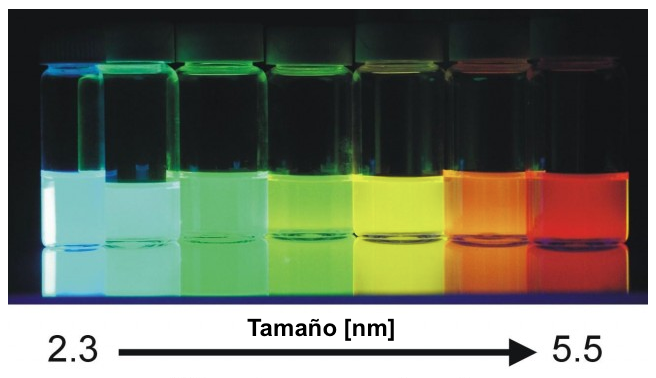
\includegraphics[width=3.2in, height=1.75in]{introduccion/qdots}
\caption{Puntos cu\'anticos. \emph{\scriptsize{Imagen de Benoit Dubertret, 2004}}}\label{fig1}
\end{figure}

A pesar de ser considerados prominentes marcadores para la obtenci\'on de im\'agenes \emph{in vivo} e \emph{in vitro}, las dudas sobre su potencial toxicidad en c\'elulas o \emph{citotoxicidad} a\'un siguen sin resolverse. 

Los puntos cu\'anticos pueden estar limitados por la presencia de metales pesados en su n\'ucleo y bajo ciertas circunstancias pueden ser t\'oxicos para las c\'elulas \cite{artiqdtox}.  Aunque la superficie de estas nanopart\'iculas se puede modificar para aumentar su biocompatibilidad o su eficiencia de emisi\'on, es dif\'icil que el di\'ametro de los puntos cu\'anticos est\'e por debajo del l\'imite de excreci\'on  renal (5.5 nm) y la toxicidad a largo plazo ser\'ia preocupante \cite{articuloQDtoxico}. 
%para adquisici\'on de im\'agenes en sistemas vivos

Otras nanopart\'iculas inorg\'anicas fluorescentes tales como los puntos de carbono, nanopart\'iculas met\'alicas y nanopar\'iculas encapsuladas con s\'ilice, normalmente no son degradables y tienen una potencial toxicidad debido a la acumulaci\'on de estos materiales en el sistema reticuloendotelial \cite{artconcluyente}. 
 
Una alternativa de marcadores fluorescentes que se presenta como soluci\'on a los problemas de citotoxicidad son las nanopart\'iculas basadas en nuevos materiales org\'anicos o con sistemas $\pi$ conjugados: materiales que presentan emisi\'on de luz inducida por agregaci\'on, pol\'imeros conjugados y mol\'eculas org\'anicas de diversos tama\~{n}os, como dendr\'imeros (macromol\'eculas). 

El desarrollo de estas nanopart\'iculas ha tenido un fuerte impacto en la microscopia de fluorescencia debido a sus caracter\'isticas fotof\'isicas: presentan grandes coeficientes de extinci\'on y de eficiencia cu\'antica de fluorescencia. Adem\'as nanopart\'iculas de pol\'imeros conjugados presentan propiedades altamente eficientes de encapsulaci\'on y transferencia de energ\'ia, mientras que las nanopart\'iculas de mol\'eculas org\'anicas peque\~{n}as presentan mayor eficiencia cu\'antica, mayor intensidad de fluorescencia y estabilidad.

Estudios sobre efectos \'opticos no lineales, en particular absorci\'on no lineal de dos fotones de estos sistemas $\pi$ conjugados,  han provocado un fuerte inter\'es debido a la flexibilidad que estos materiales poseen para modificar sus estructuras a nivel molecular y optimizar su respuesta no lineal. Pueden ser utilizados como marcadores en t\'ecnicas de microscop\'ia multifot\'on, como en microscop\'ia de barrido l\'aser de dos fotones, en la cual el fluor\'oforo es excitado con la absorci\'on no lineal de dos fotones. Esta t\'ecnica presenta ventajas ante la microscop\'ia de fluorescencia inducida por la absorci\'on de un fot\'on, como mayor profundidad de penetraci\'on en tejidos por la relativa transparencia que \'estos presentan ante radiaci\'on infrarroja y la confinaci\'on de la destrucci\'on fotoqu\'imica al volumen focal, entre otras.

Aunque la mayor\'ia de este tipo de materiales org\'anicos son hidrof\'obicos y los marcadres biocompatibles deben ser solubles en agua, hay m\'etodos que desarrollan suspensiones acuosas de nanopart\'iculas, mediante la modificaci\'on de su superficie o funcionalizaci\'on. El recubrimiento de las nanopart\'iculas es crucial para determinar sus propiedades, puede regular la estabilidad, solubilidad y orientaci\'on; puede aumentar la biocompatibilidad y permitir bioconjugaciones (uni\'on a biomol\'eculas, que pueden conferir a las nanopart\'iculas selectividad hacia l\'ineas celulares espec\'ificas o hacia estructuras espec\'ificas dentro de la c\'elula).  


\section{Nanopart\'iculas org\'anicas funcionalizadas con PEG utilizadas como marcadores}

Cuando la modificaci\'on de superficie en las nanopart\'iculas se realiza mediante la adhesi\'on de grupos funcionales, al proceso se le conoce como \emph{funcionalizaci\'on}.  

El polietilenglicol (PEG) es un poli\'eter de baja toxicidad que puede ser sintetizado en una gran variedad de pesos moleculares. El PEG ha sido ampliamente utilizado en aplicaciones cl\'inicas; puede encapsular diversos fluor\'oforos y medicamentos, facilitando la entrega de f\'armacos en sistemas vivos.

La funcionalizaci\'on de nanopart\'iculas org\'anicas con PEG facilita la conjugaci\'on con anticuerpos, enzimas y prote\'inas. De esta manera, las nanopart\'iculas funcionalizadas pueden ser utilizadas como marcadores selectivos y ubicar c\'elulas espec\'ificas como c\'elulas cancer\'igenas en la adquisici\'on de im\'agenes.

Utilizar PEG en nanopart\'iculas org\'anicas para desarrollar marcadores biocompatibles tiene diversos beneficios; puede provocar que las nanopart\'iculas tengan una vida media m\'as prolongada en la sangre y menor absorci\'on en el h\'igado en comparaci\'on con las naopart\'iculas que no tienen este recubrimiento \cite{drugsdeliv}, adem\'as el PEG promueve la eliminaci\'on de nanopart\'iculas del torrente sangu\'ineo mediante el sistema reticuloendotelial, es decir, no permite su degradaci\'on en la sangre.

\section{Objetivos de este trabajo}

Los objetivos principales del trabajo fueron:

\begin{description}
\item 1) Estudiar la emisi\'on de luz inducida por uno y dos fotones en nanopart\'iculas org\'anicas funcionalizadas con PEG, utilizando para ello nuevos materiales org\'anicos no lineales.
\item 2) Comparaci\'on de propiedades no lineales entre soluciones y suspensiones acuosas de nanopart\'iculas del material precursor hidrof\'obico.
\item 2) Estudiar la transferencia de energ�a de resonancia F�rster en suspensiones acuosas de nanopart�culas.
\item 3) Aplicar las nanopart\'iculas estudiadas como marcadores de l\'ineas celulares y obtener im\'agenes con un microscopio de epifluorescencia.
\end{description}

En la funcionalizaci\'on realizada en este trabajo se utiliz\'o un PEG como agente estabilizador en las suspensiones acuosas de nanopart\'iculas. 


